\documentclass[11pt,a4paper]{article}
\usepackage[utf8]{inputenc}
\usepackage[spanish]{babel}
\usepackage{graphicx}
\usepackage{amsmath,amssymb,amsfonts}
\usepackage{mathtools}
\usepackage{geometry}
\usepackage{xcolor}
\usepackage{hyperref}
\usepackage{booktabs}
\usepackage{enumitem}
\usepackage{fancyhdr}
\usepackage{titlesec}
\usepackage{microtype}
\usepackage{float}
\usepackage{listings}
\usepackage{color}

% Establecer márgenes
\geometry{a4paper, margin=1in, top=1.2in, headheight=15pt}

% Configurar hipervínculos
\hypersetup{
    colorlinks=true,
    linkcolor=blue,
    filecolor=blue,
    citecolor=blue,
    urlcolor=blue,
    pdftitle={Práctica 1},
    pdfauthor={Renato Bedriñana Cárdenas, Hugo Blanco Demelo},
    pdfsubject={Práctica 1 - Sampling and Quantization},
}

% Configuración de encabezado y pie de página
\pagestyle{fancy}
\fancyhf{}
\fancyhead[L]{\footnotesize Práctica 1}
\fancyhead[R]{\footnotesize Sampling and Quantization}
\fancyfoot[C]{\thepage}
\renewcommand{\headrulewidth}{0.4pt}
\renewcommand{\footrulewidth}{0.4pt}

% Configuración para código fuente
\definecolor{codegreen}{rgb}{0,0.6,0}
\definecolor{codegray}{rgb}{0.5,0.5,0.5}
\definecolor{codepurple}{rgb}{0.58,0,0.82}
\definecolor{backcolour}{rgb}{0.95,0.95,0.95}

\lstset{
    backgroundcolor=\color{backcolour},
    commentstyle=\color{codegreen},
    keywordstyle=\color{magenta},
    stringstyle=\color{codepurple},
    basicstyle=\ttfamily\small,
    breakatwhitespace=false,
    breaklines=true,
    captionpos=b,
    keepspaces=true,
    numbersep=5pt,
    showspaces=false,
    showstringspaces=false,
    showtabs=false,
    tabsize=2
}

% Formato de títulos
\titleformat{\section}
  {\normalfont\large\bfseries\color{blue!70!black}}
  {\thesection}{1em}{}
\titleformat{\subsection}
  {\normalfont\normalsize\bfseries\color{blue!60!black}}
  {\thesubsection}{1em}{}

% Espacio después de secciones
\titlespacing*{\section}{0pt}{3.5ex plus 1ex minus .2ex}{2.3ex plus .2ex}
\titlespacing*{\subsection}{0pt}{3.25ex plus 1ex minus .2ex}{1.5ex plus .2ex}

% Definición de comandos para matemáticas
\newcommand{\dB}{\text{dB}}
\newcommand{\dBFS}{\text{dBFS}}

% Información del documento
\title{\vspace{-1.5cm}\Large\textbf{Práctica 1: Sampling and Quantization}}
\author{\normalsize Renato Bedriñana Cárdenas \and \normalsize Hugo Blanco Demelo}
\date{\normalsize\today}

\begin{document}

\maketitle
\section{Task 1}
\textbf{Question: Give your interpretation of the resulting graphs. Do the quantization levels correspond with the values you had expected?}

\vspace{0.5cm}
We represent the original continuous signal x (blue) and the 2 quantized version using 2 (red) and 4 (yellow) bits. As expected, the 2 bit quantization produces fewer discrete levels than the 4 bits quantization. Increase the number of bits decreases $\Delta$, resulting in smaller steps and a quantized signal that follows the input more closely.

\vspace{1cm}
\textbf{Question: For both cases, represent the quantization error as a function of input amplitude in the range $[-7, +7]$ and comment on your results. Is this error always within the $[-\Delta /2, +\Delta /2]$ interval?}

\vspace{0.5cm}
The magnitude of the error decreases as the number of bits increases, since a smaller quantization step 
$\Delta$ reduces the maximum deviation between the input and its quantized version.
The $[-\Delta /2, +\Delta /2]$ in each case is as follows:
\begin{itemize}
    \item For N = 2 the $\Delta$ value we get is $\Delta = 3.5$, so the interval should be $[-1.75, 1.75]$.
    \item For N = 4 the $\Delta$ value we get is $\Delta = 0.875$, so the interval should be $[-0.4375, 0.4375]$.
\end{itemize}
In both cases, the error remains bounded within the theoretical interval $[-\Delta /2, +\Delta /2]$.

\begin{figure}[H]  % H is fot NOT letting latex insert the image in another place
    \centering
    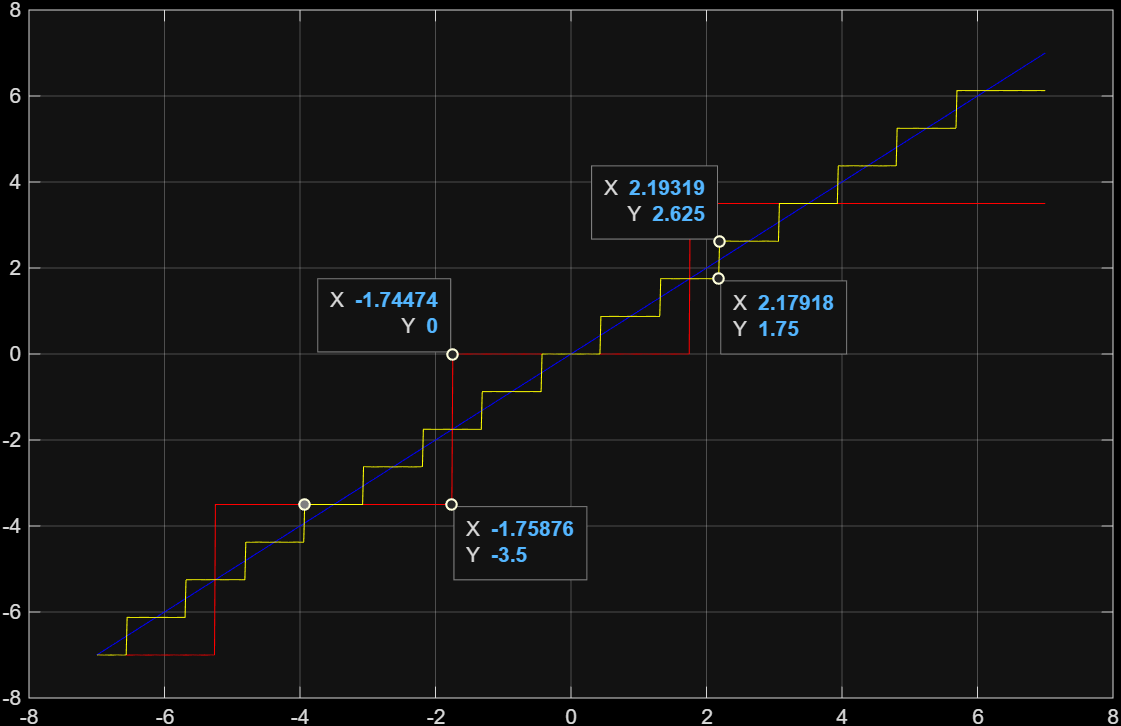
\includegraphics[width=1\textwidth]{img/task1_2.png}
    % \caption{Description of your image}
    \label{fig:task1_2}
\end{figure}

\begin{figure}[H]
    \centering
    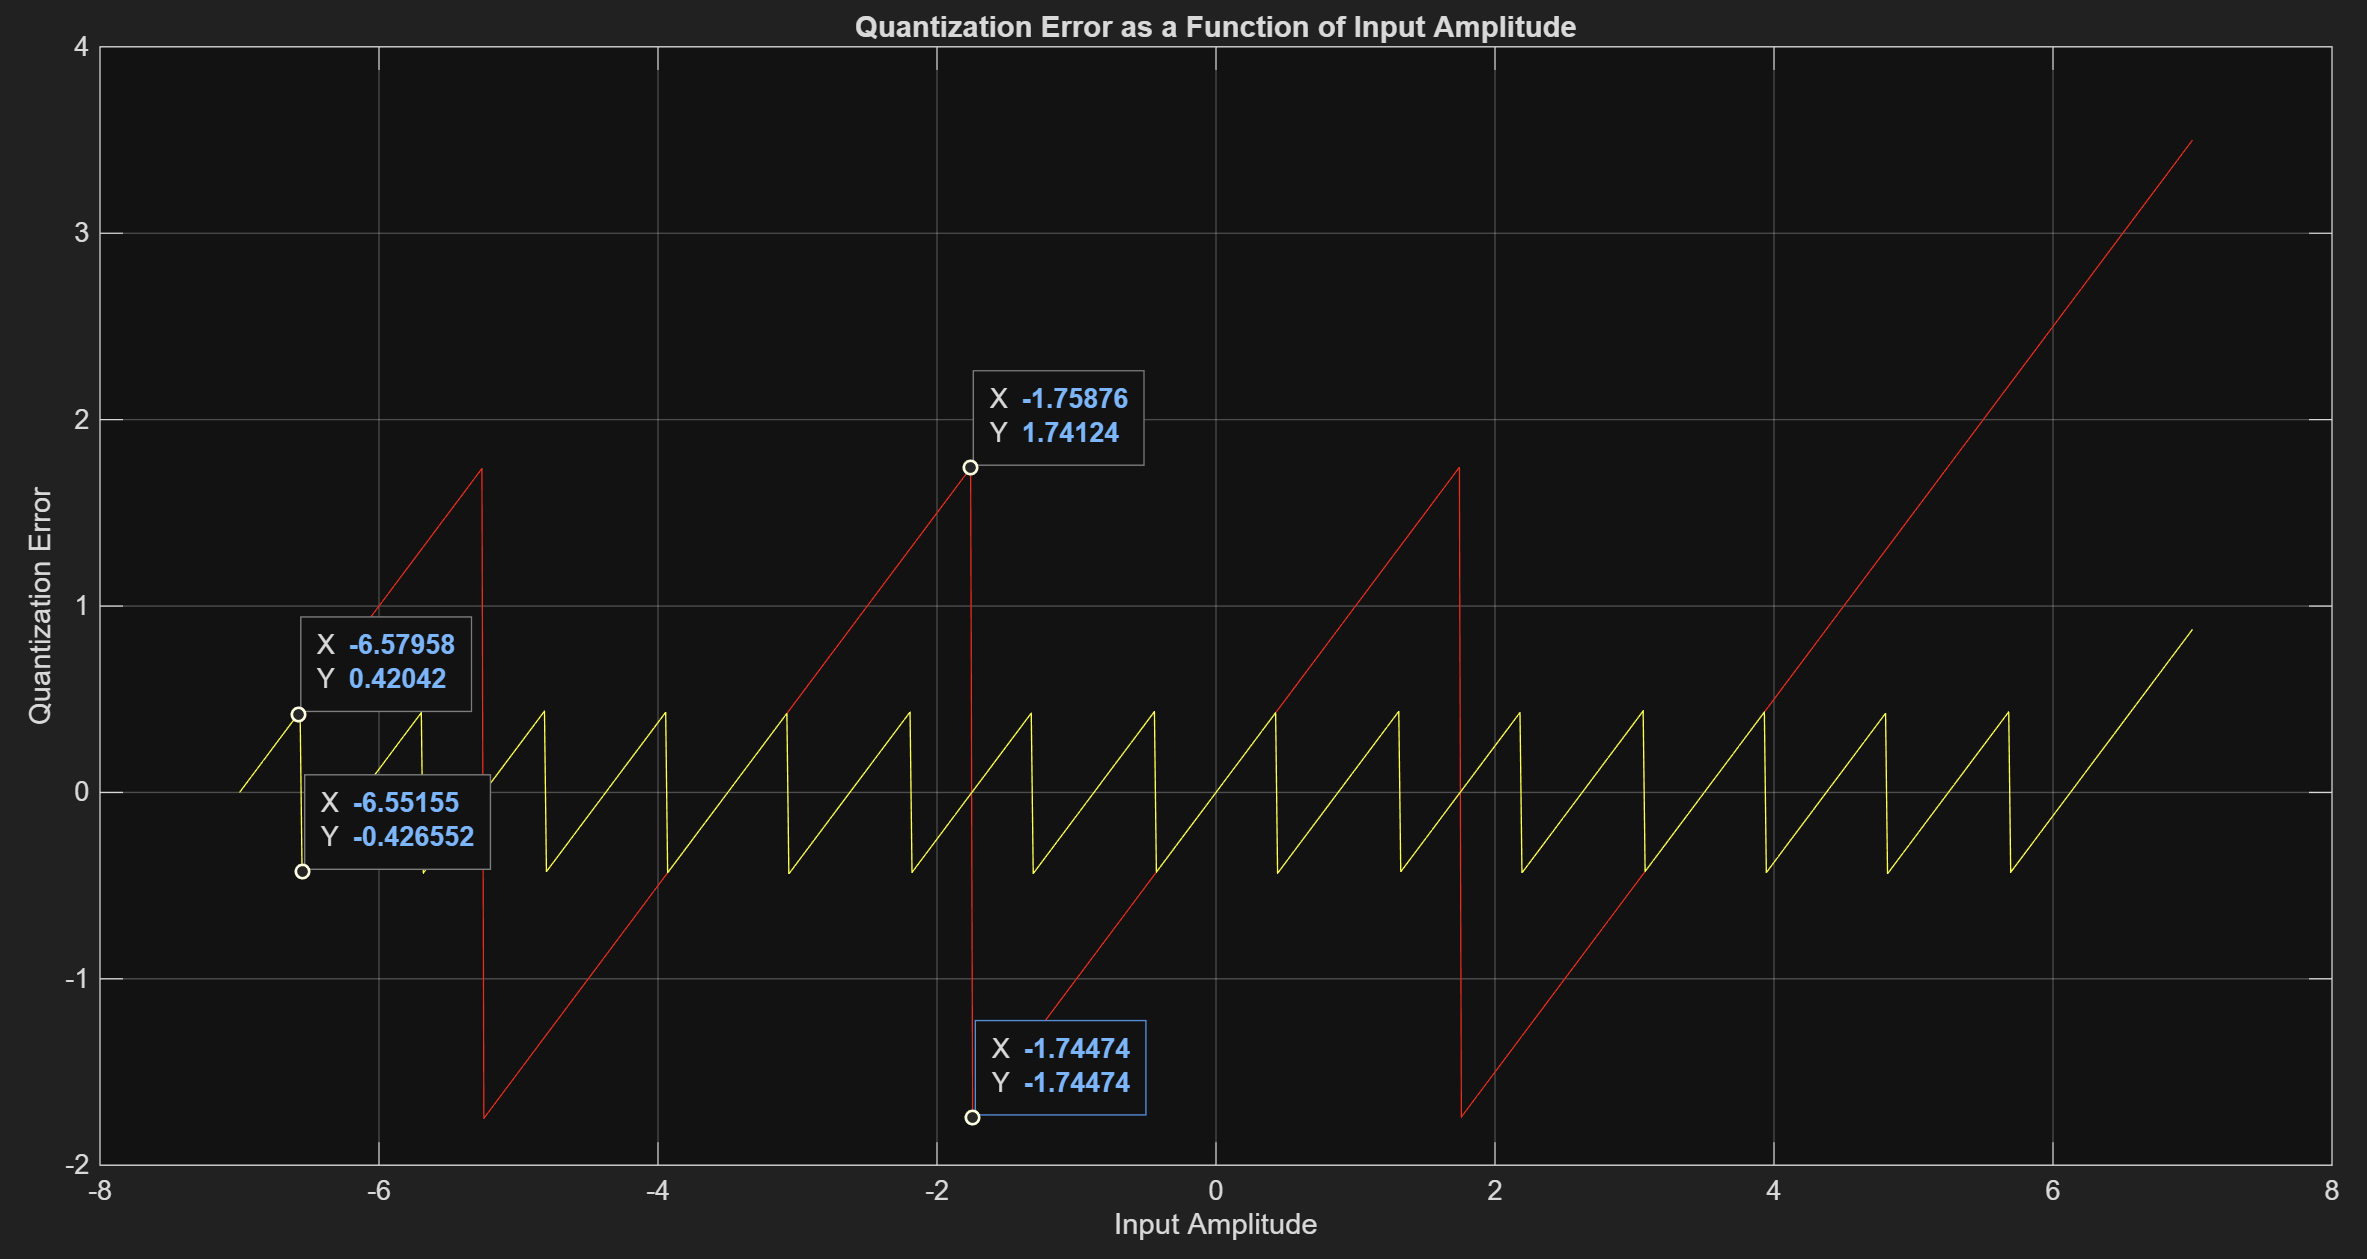
\includegraphics[width=1\textwidth]{img/task1_2_2.png}
    % \caption{Description of your image}
    \label{fig:task1_2_2}
\end{figure}

\section{Task 2}
\textbf{Question: Assume a full-scale sinusoidal input and plot the histogram of the quantization error. Do you observe what you expected, or not?}

\vspace{0.5cm}
$\Delta= \frac{2*FS}{2^N} = 0.0098$, so the $[-\frac{\Delta}{2}, +\frac{\Delta}{2}]$ interval should be $[-0.0049, +0.0049]$.
In the histogram we can see that in that interval the error is uniformly distributed, but there is an error tail in the positive extreme.
It means that there is \textbf{clipping} in the positive.

\begin{figure}[H]
    \centering
    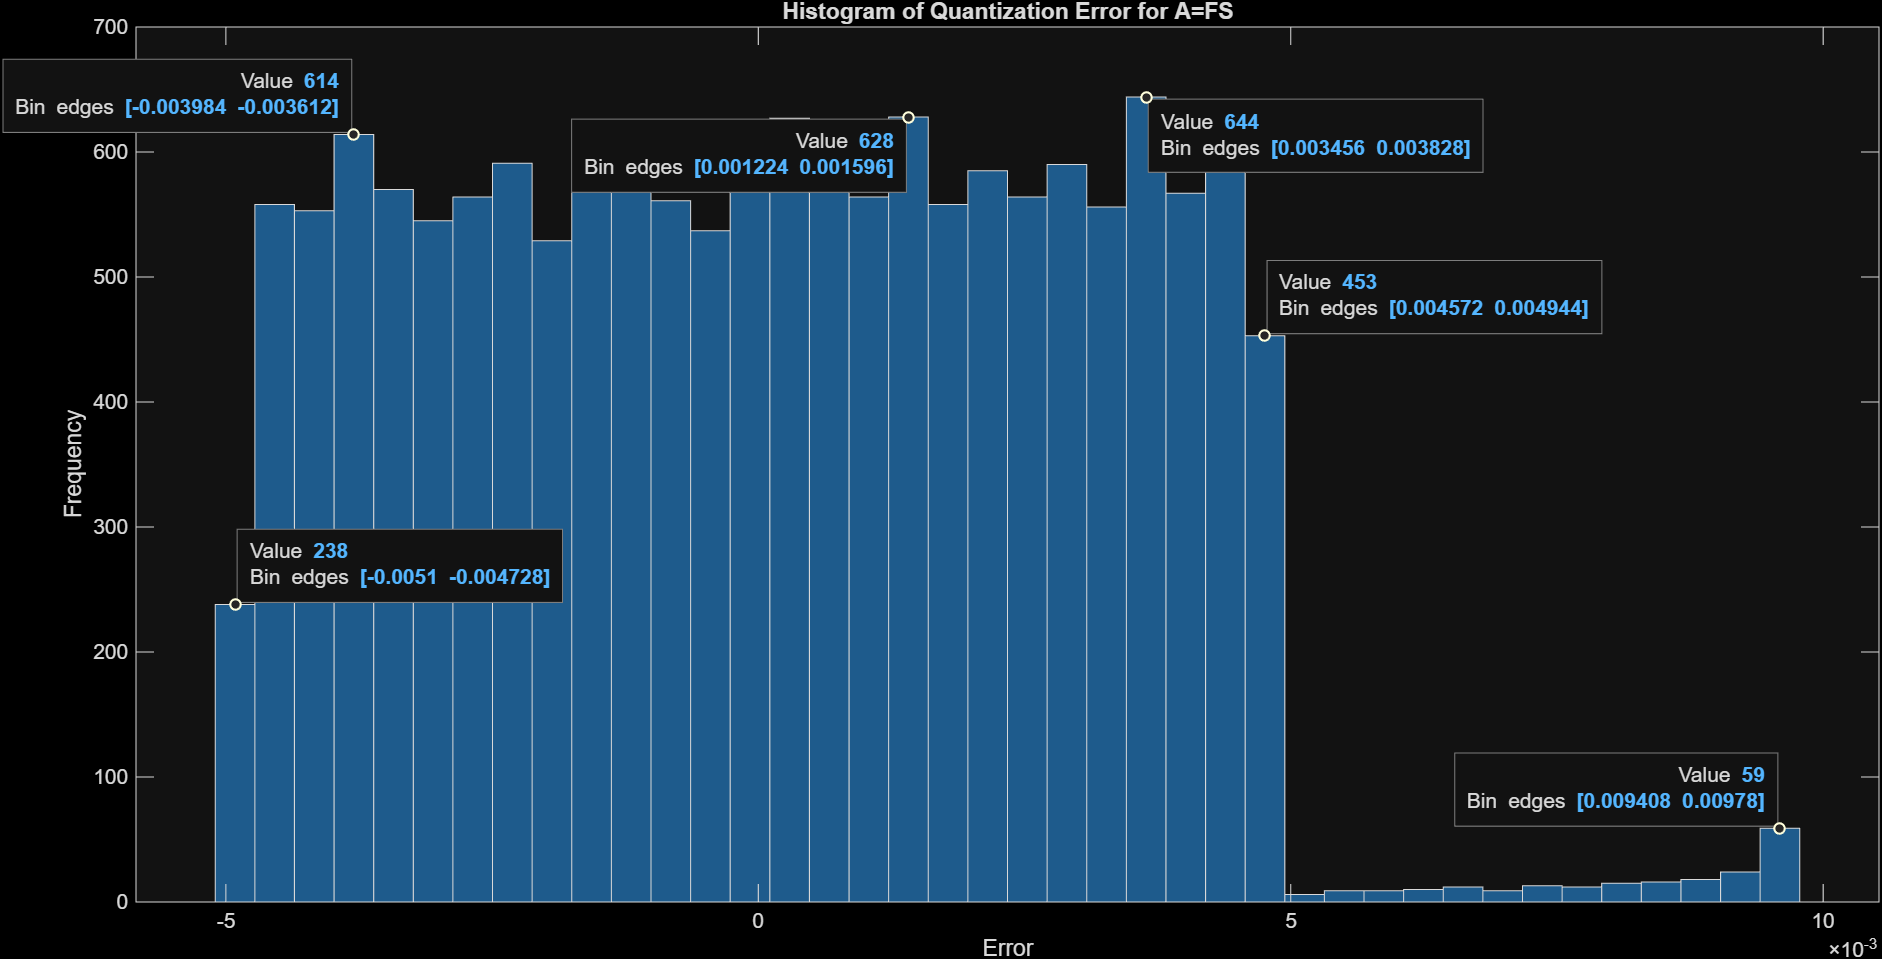
\includegraphics[width=1\textwidth]{img/task2_1.png}
    % \caption{Description of your image}
    \label{fig:task2_1}
\end{figure}

\vspace{1cm}
\textbf{Question: Explain the operation of the Matlab command var. Estimate the variance of the quantization error using var,
    and compare it to its theoretical value. Estimate the value (in dB) of the Signal to-Quantization Noise Ratio (SQNR)
    and compare it to its theoretical value (1).
}

\vspace{0.5cm}
The MATLAB command \texttt{var} computes the variance of a set of values. For a vector $x$, it calculates:
$\text{var}(x) = \frac{1}{n-1}\sum_{i=1}^n (x_i - \bar{x})^2$, where $\bar{x}$ is the mean of the values in $x$.

ADD
\begin{figure}[H]
    \centering
    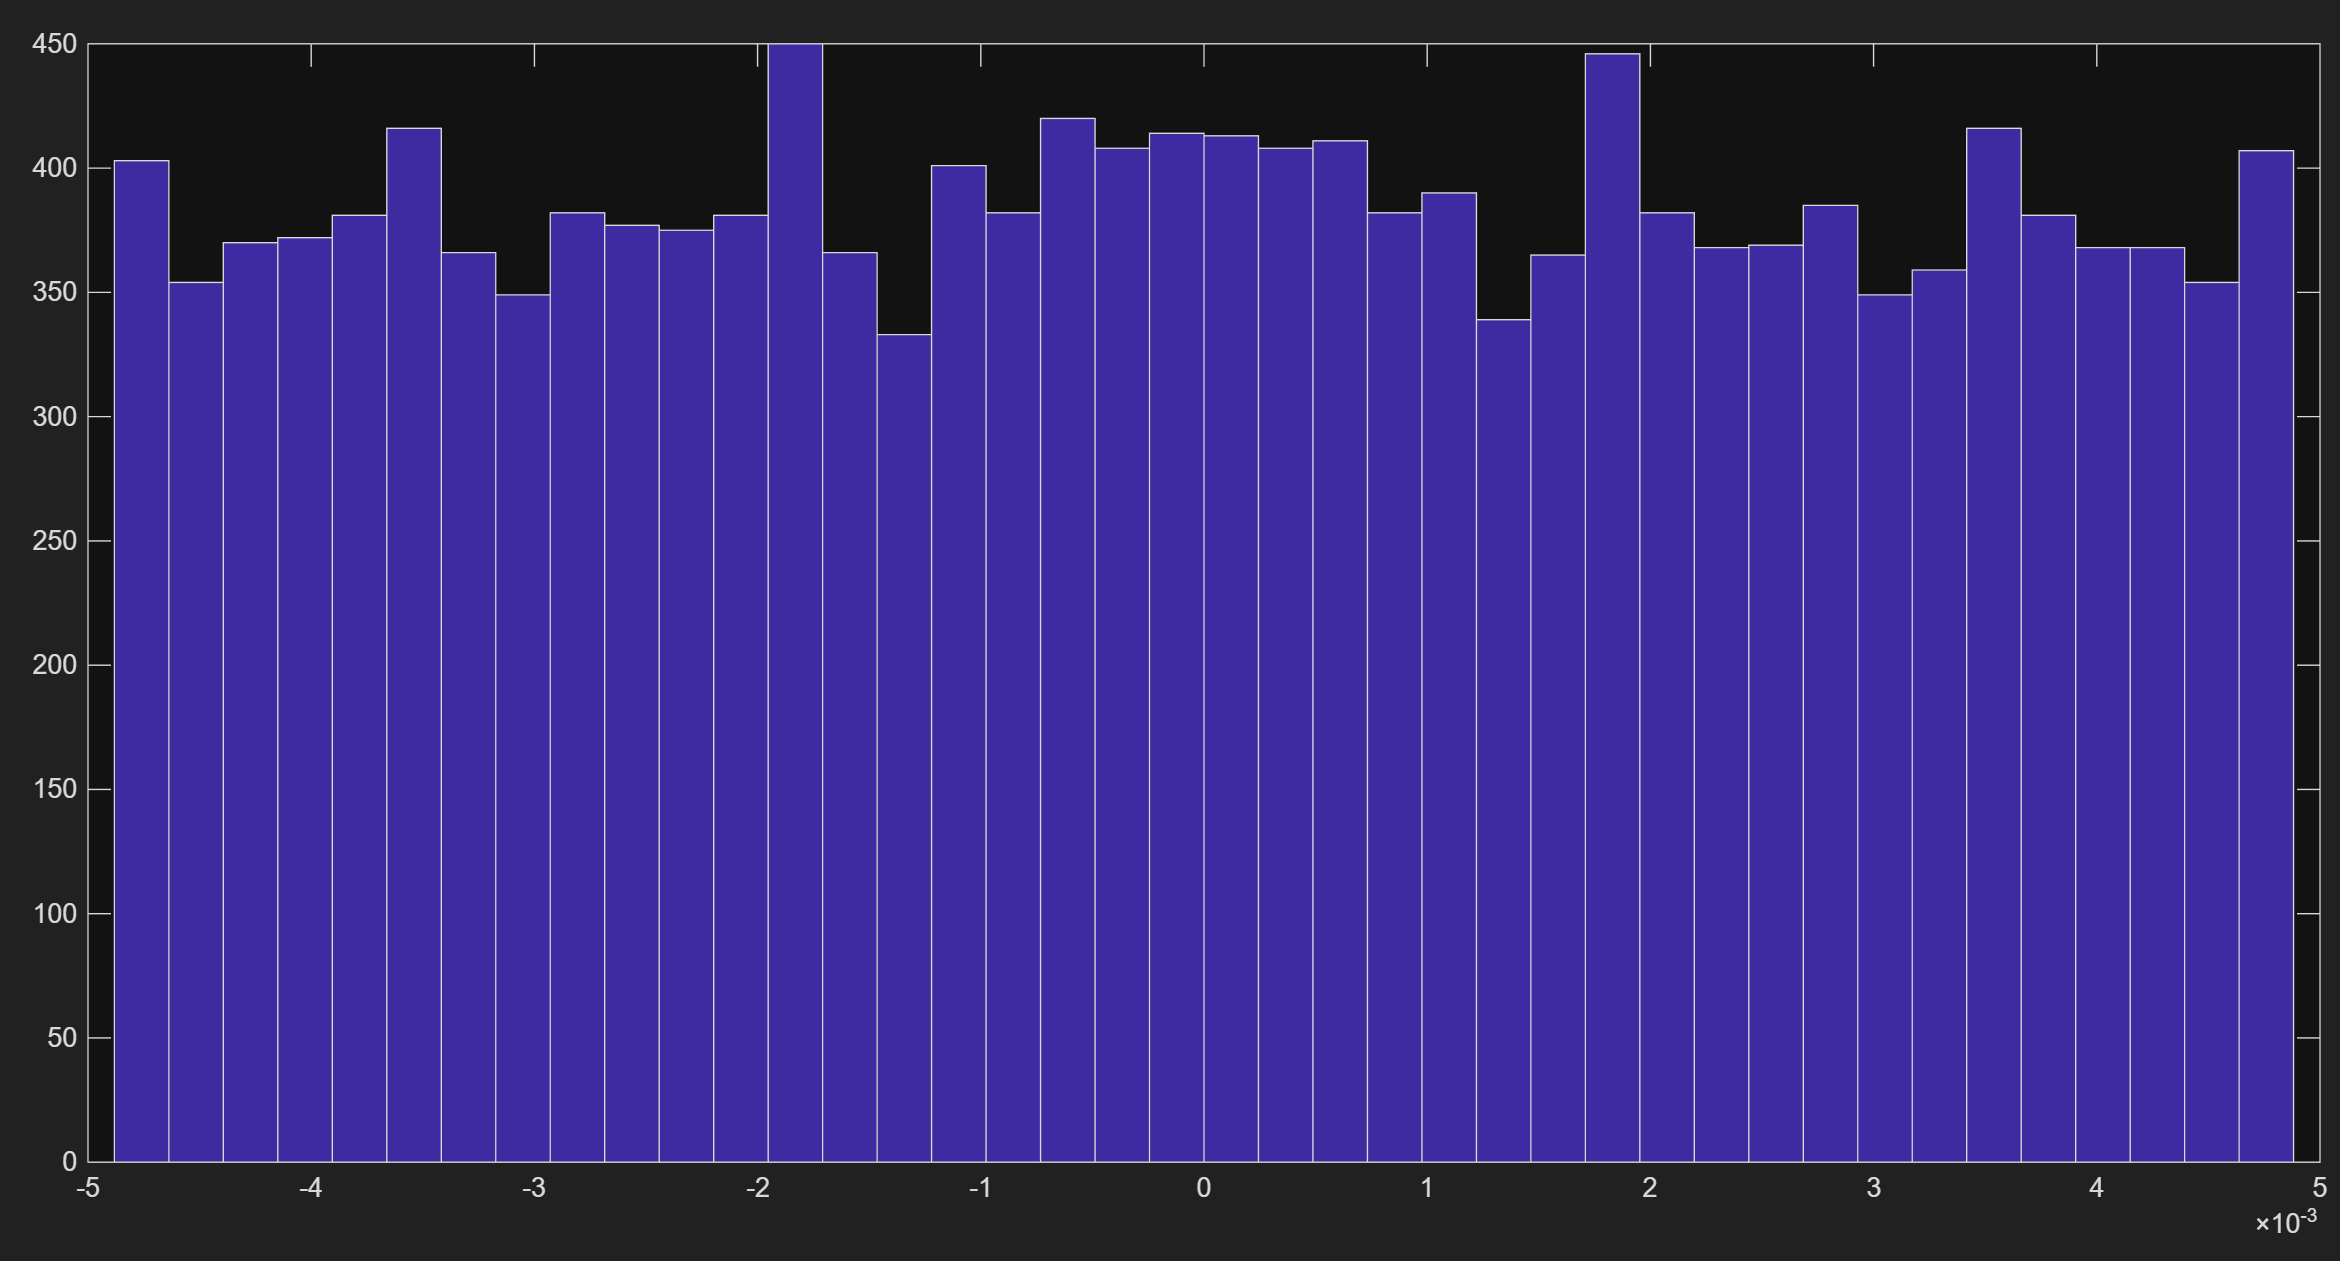
\includegraphics[width=1\textwidth]{img/task2_2.png}
    % \caption{Description of your image}
    \label{fig:task2_2}
\end{figure}

\vspace{1cm}
\textbf{Question: Repeat the previous steps for sinusoids with different amplitudes, and with decreasing resolutions
    of 12, 10, 8, 6 and 4 bits, in order to fill Table 1, rounding the SQNR values (in dB) to two
    decimal places. Comment on your results.
}

\vspace{0.5cm}
\begin{table}[H]
    \centering
    \begin{tabular}{|c||c|c|c|c|c|c|c|c|}
        \hline
                    & \multicolumn{2}{c|}{$A=0.5\cdot\text{\tt FS}$} & \multicolumn{2}{c|}{$A=0.75\cdot\text{\tt FS}$} & \multicolumn{2}{c|}{$A=\text{\tt FS}$} & \multicolumn{2}{c|}{$A=1.03\cdot\text{\tt FS}$}                                         \\
        \cline{2-9} & \multicolumn{2}{ |c| }{SQNR (dB)}              & \multicolumn{2}{ |c| }{SQNR (dB)}               & \multicolumn{2}{ |c| }{SQNR (dB)}      & \multicolumn{2}{ |c| }{SQNR (dB)}                                                       \\
        \hline
        $N$         & theory                                         & measured                                        & theory                                 & measured                                        & theory & measured & theory & measured \\
        \hline\hline
        12          & 61.96                                          & 62.02                                           & 67.98                                  & 68.03                                           & 71.50  & 71.54    & 74.00  & 73.70    \\
        \hline
        10          & 49.92                                          & 50.01                                           & 55.94                                  & 56.01                                           & 59.46  & 59.53    & 61.96  & 61.56    \\
        \hline
        8           & 37.88                                          & 38.07                                           & 43.90                                  & 44.04                                           & 47.42  & 47.53    & 49.92  & 49.15    \\
        \hline
        6           & 25.84                                          & 26.22                                           & 31.86                                  & 32.13                                           & 35.38  & 35.60    & 37.88  & 36.52    \\
        \hline
        4           & 13.80                                          & 14.59                                           & 19.82                                  & 20.37                                           & 23.34  & 23.78    & 25.84  & 23.63    \\
        \hline
    \end{tabular}
    \caption{Pertaining to Task 2.}
    \label{tab:task2}
\end{table}

\section{Task 3}
\textbf{Question: Suppose that you have an N-bit A/D converter with tunable FS, and you know that your input samples follow
    a symmetric triangular pdf in some interval $[-x_0,x_0]$. Intuitively, how would you set the FS value of your converter?
    What would the resulting rms value $\sigma_x$ in dBFS be?
}

\vspace{0.5cm}
If you set $FS < x_0$ any imput $|x|$ greater than FS will be clipped. If $FS > x_0$,we would be wasting the converter's since the signal would never
reach the limits. Therefore, the value of FS should be $x_0$.

$\sigma_x = \sqrt{var(x)} = \frac{x_0}{\sqrt{6}}$ and in dBFS would be $20\log_{10}(1/\sqrt{6}) = -7,78$ dBFS.

\vspace{1cm}
\textbf{Question: Explain how to generate in Matlab samples of a random variable following a symmetric triangular pdf with
    zero mean and rms value $\sigma_0$. Check the histogram and use the commands mean and var to validate your approach
}

\vspace{0.5cm}
We have two options to do it:
\begin{itemize}
    \item Option 1: We can do it using \textit{makedist} function. To do it, we can use the following code:
          \begin{lstlisting}[language=Matlab]
            x0 = 2;
            A = -x0; B = 0; C = +x0; % simetria = media 0

            pd = makedist('Triangular','A',A,'B',B,'C',C);
            N = 100000;
            samples = random(pd, N, 1);

            % comprobaciones rapidas
            emp_mean = mean(samples);
            emp_var = var(samples);
            emp_desv_std = std(samples);

            % valores teoricos
            % theo_mean = 0; % simetria centrado en 0
            theo_var = (A^2 + B^2 + C^2 - A*B - A*C - B*C)/18;
            rms = 20*log10(sqrt(theo_var)/x0);

            fprintf('Theorical mean: 0; emp mean: %.2f\n',emp_mean);
            fprintf('Theorical var: %.2f; emp var: %.2f\n',theo_var,emp_var);
            fprintf('Sigma value: %.2f\n',sqrt(theo_var));
            fprintf('rms value in dBFS: %.2f\n',rms)

            % ver histograma y pdf teorica
            xgrid = linspace(A,C,500)';
            figure
            histogram(samples,100,'Normalization','pdf')
            hold on
            plot(xgrid, pdf(pd,xgrid), 'LineWidth',1.5)
            title('Triangular (media 0) -- muestras vs PDF')
            hold off
        \end{lstlisting}
    \item Option 2: we can generate samples of a random variable following a symmetric triangular pdf as the sum of two independent
          random variables $X_1$ and $X_2$  from a uniform distribution.
          we can doit as follows: REVISAR!!
          \begin{lstlisting}[language=Matlab]
            x0=2;
            sigma0 = x0/sqrt(2);
            N = 100000;
            
            c = sigma0 * sqrt(3/2);

            x1 = (2 * rand(N, 1) - 1) * c;
            x2 = (2 * rand(N, 1) - 1) * c;

            y = x1 + x2;

            sample_mean = mean(y);
            sample_var = var(y);
            sample_rms = std(y);

            fprintf('--- Validation ---\n');
            fprintf('Target Mean: 0.0\n');
            fprintf('Sample Mean: %f\n\n', sample_mean);

            fprintf('Target Variance (sigma0^2): %f\n', sigma0^2);
            fprintf('Sample Variance: %f\n\n', sample_var);

            fprintf('Target RMS (sigma0): %f\n', sigma0);
            fprintf('Sample RMS: %f\n\n', sample_rms);

            figure;
            histogram(y, 100, 'Normalization', 'pdf', 'DisplayName', 'Generated Samples');
            grid on;
            hold on;

            a = 2*c;
            x_pdf = linspace(-a, a, 400);
            y_pdf = (1/a) * (1 - abs(x_pdf)/a);
            plot(x_pdf, y_pdf, 'r-', 'LineWidth', 2.5, 'DisplayName', 'Theoretical PDF');

            title('Symmetric Triangular Distribution');
            xlabel('Random Variable Value');
            ylabel('Probability Density Function (PDF)');
            legend;
            hold off;
        \end{lstlisting}
\end{itemize}

\vspace{1cm}
\textbf{Question: Take $10\cdot 2^{10}$ of these triangularly distributed samples, quantize them, and estimate the SQNR empirically
    for $N=$ 3, 4, 5 and 6 bits. Do this for $\sigma_x$ varying in the range $[-50, 0]$ dBFS and in steps of $0.1$ dBFS. Plot the
    resulting curves (SQNR in dB vs. $\sigma_x$ in dBFS) along with the theoretical expression
    \begin{equation}\label{eq:sqnr}
        {\rm SQNR} = 6.02 N + 4.77-20\log_{10}\frac{\rm FS}{\sigma_x} \qquad \mbox{(dB).}
    \end{equation}
    Are there any differences between the theoretical and empirical curves? If so, how do you explain them?}
\vspace{0.5cm}
ADD

\vspace{1cm}
\textbf{Question: In view of your results, what are the optimum values (regarding SQNR) of $\sigma_x$ (in dBFS), and for the different resolutions analyzed (3 to 6 bits)?
    Does this agree with your intuition (see first point above)?
}
\vspace{0.5cm}

\end{document}